\vspace{10pt}

{\centering\subsection*{梁好:游万达海洋馆}}

\addcontentsline{toc}{subsection}{梁好:游万达海洋馆}

\renewcommand{\leftmark}{梁好:游万达海洋馆}

\begin{figure}[htbp]

\centering

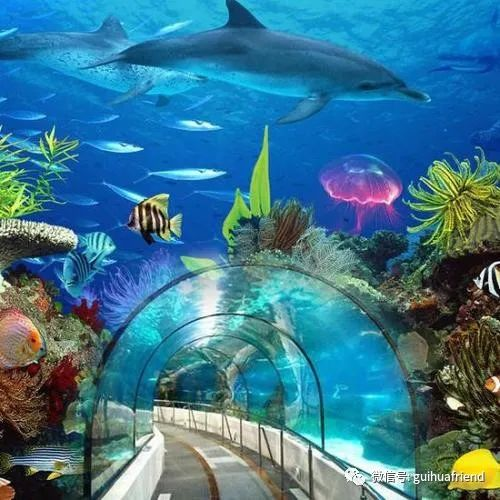
\includegraphics[width = .5\textwidth]{./ch/14.jpg}

\end{figure}



五一假期的时候,我去万达广场的海洋馆玩。

一走进大门,就有一股闷热的感觉。向西北方向走,我突然看到了上百个亮点,在水中飘动,像一盏盏灯,在水中飘荡,走进后发现原来是水母。它那身体看上去那么柔软,看着像一朵朵蘑菇。触手随着水飘荡,像丝线一般,只见它触手缩着,随后触手就会猛的一伸开,有时候还会左右摇摆。它们还有各种各样的颜色呢!

参观完水母,再往右走,你会你会发现一些很奇特的生物,它们不可以自己移动,只能靠着水流移动,但它们却可以活动,最重要的是它的下面竟长着植物,这让我感到世界是多么神奇呀!但是我也不知道它是什么。

看完了奇怪的生物,又来到一个大的水箱面前,只见一只很扁的鱼出现在眼前,我拍了一下水箱,想吓吓他,结果它立马变得鼓鼓的,还有很多的利刺,我没把它吓到,结果它还把我给吓到了,真是好笑。

参观完刺豚后,我又去参观传说中的魔鬼鱼。在看到魔鬼鱼之前,我就被他这个名字惊恐到了。到了之后,我发现他并没有那么可怕,他两旁的鱼皮往上翘起,眼睛旁还有一个洞,身上黑中带白,后面还有一条根电线杆一样的尾巴……

这就是海洋馆的风景,真是看也看不完,希望你也能去细细观看。





\vspace{10pt}



作者:四(1)班 梁好



指导老师:周瑞



投稿:2021年5月27日



发表:2021年5月28日












                



\vspace{10pt}

\hline



